\documentclass[conference]{IEEEtran}
\IEEEoverridecommandlockouts

\usepackage{cite}
\usepackage{amsmath,amssymb,amsfonts}
\usepackage{graphicx}
\usepackage{textcomp}
\usepackage{xcolor}
\usepackage{booktabs}
\usepackage{array}
\usepackage{url}
\usepackage{tikz}
\usetikzlibrary{arrows.meta,positioning,shapes.geometric}
\usepackage{pgfplots}
\pgfplotsset{compat=1.16}

\def\BibTeX{{\rm B\kern-.05em{\sc i\kern-.025em b}\kern-.08em
    T\kern-.1667em\lower.7ex\hbox{E}\kern-.125em X}}

\begin{document}

\title{Does Fine-Tuning Help? A Comparative Study of Cloud, Base and LoRA-Fine-Tuned Language Models with Retrieval for Operating Systems Question Answering}

\author{\IEEEauthorblockN{First Author}
\IEEEauthorblockA{\textit{Department of Computer Science} \\
\textit{Your Institution}\\
City, Country \\
email@example.com}
\and
\IEEEauthorblockN{Second Author}
\IEEEauthorblockA{\textit{Department of Computer Science} \\
\textit{Your Institution}\\
City, Country \\
email@example.com}
}

\maketitle

\begin{abstract}
We study whether adapting a small language model to a course textbook, and adding retrieval, can match a much larger cloud model for operating-systems (OS) question answering. We built an OS tutoring pipeline over a standard textbook, a 762-example instruction dataset, and a LoRA adapter for Qwen2.5-1.5B-Instruct, and compared six systems: cloud model, base Qwen and fine-tuned Qwen, each with and without retrieval. After removing 15 of 32 gold questions that closely match training examples, we scored the remaining 17 with RAGAS (LLM judge), and measured calculation accuracy on 27 newly generated problems whose answers are computed by simulation. The cloud model with retrieval was the most faithful system (0.61 versus 0.32 for fine-tuned Qwen with retrieval). Fine-tuning did not improve the text metrics: compared with its own base model, the fine-tuned model had lower answer relevancy (by 0.13 without and 0.07 with retrieval) and no detectable gain in faithfulness. On calculations the cloud model answered 22 of 27 correctly, while fine-tuned and base Qwen answered 1 and 0 under a strict criterion (8 and 4 under a lenient one; difference not significant). We report these negative and inconclusive results together with the data-quality problems we found and corrected, the train/test overlap check, and the limitations of a small, single-judge study.
\end{abstract}

\begin{IEEEkeywords}
retrieval-augmented generation, LoRA, small language models, fine-tuning, educational question answering, operating systems, RAGAS, evaluation
\end{IEEEkeywords}

%==============================================================
\section{Introduction}
Students of operating systems increasingly ask general chatbots about course material. Answers are fluent but not tied to the course textbook, and small errors are hard for novices to spot. Retrieval-augmented generation (RAG)~\cite{lewis2020rag} grounds answers in retrieved passages, and parameter-efficient fine-tuning such as LoRA~\cite{hu2022lora} and QLoRA~\cite{dettmers2023qlora} makes it feasible to adapt a small model on modest hardware, which would allow a tutor to run locally and offline.

We ask a plain empirical question: \emph{given a textbook, does LoRA fine-tuning of a 1.5B-parameter model add measurable value over the same model without fine-tuning, and how far is the result from a larger cloud model?} We built the pipeline, fixed the evaluation problems we met along the way, and report the outcome, including where it disappointed.

Our contributions are:
\begin{enumerate}
  \item A \textbf{comparative study} of six configurations (cloud, base Qwen, fine-tuned Qwen; each with and without retrieval) on questions with no near-duplicate in the fine-tuning data, with paired confidence intervals.
  \item A 762-example OS \textbf{instruction dataset} (seven categories, 40 refusal examples, simulator-computed numerical answers) and the \textbf{LoRA adapter} trained on it, documented honestly including its weaknesses.
  \item A judge-free \textbf{calculation benchmark} with simulator-computed ground truth.
  \item An \textbf{evaluation protocol} with a train/test overlap check, and a record of pitfalls (decoding penalties, memory leakage, empty or error answers stored as answers, wrong reference answers, judge quotas) that can silently change results.
\end{enumerate}

%==============================================================
\section{Related Work}
\textbf{RAG.} Lewis et al.~\cite{lewis2020rag} combine a generator with a retrieval index; surveys~\cite{gao2023ragsurvey} catalogue later retrieval, chunking and reranking variants. We use a plain dense-retrieval baseline shared by all RAG systems.

\textbf{Parameter-efficient fine-tuning.} LoRA~\cite{hu2022lora} trains low-rank updates to frozen weights; QLoRA~\cite{dettmers2023qlora} does so on a 4-bit base. Our base model comes from the Qwen2.5 family~\cite{qwen25}.

\textbf{Evaluation.} RAGAS~\cite{es2024ragas} defines reference-light metrics for faithfulness, answer relevancy and context quality using an LLM judge; LLM judges are convenient but biased~\cite{zheng2023judge}, and hallucination is well documented~\cite{ji2023hallucination}. We therefore add a judge-free calculation benchmark and treat judge scores as indicative.

%==============================================================
\section{System and Artifacts}

\subsection{Retrieval}
The knowledge base is one OS textbook PDF~\cite{galvin}, parsed with PyMuPDF and split into 1000-character chunks with 200 characters of overlap (4{,}330 chunks), embedded with BAAI/bge-small-en-v1.5~\cite{xiao2023cpack} and stored in Qdrant. At query time the top three chunks with similarity at least 0.55 are retrieved. All RAG systems share this retriever.

\subsection{Generators}
\textbf{Local.} Qwen2.5-1.5B-Instruct~\cite{qwen25} in 32-bit precision on CPU, with or without our LoRA adapter. Decoding: sampling with temperature 0.1, top-$p$ 0.85, repetition penalty 1.1, at most 256 new tokens, with a concise tutor system prompt. The base-model variants bypass the adapter at inference, so prompt, decoding, retriever and machine are identical.

\textbf{Cloud.} An open-weight 20B model (\texttt{openai/gpt-oss-20b}~\cite{gptoss}) through the Groq API, using the repository's RAG prompt.

\begin{figure}[t]
\centering
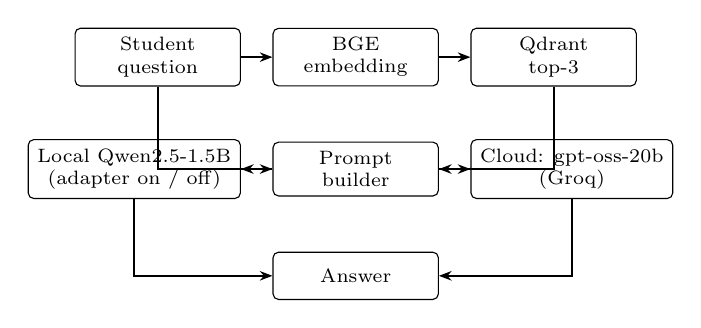
\begin{tikzpicture}[
  node distance=4mm,
  box/.style={draw, rounded corners=2pt, minimum height=6mm, minimum width=2.1cm, align=center, font=\scriptsize},
  arr/.style={-{Stealth[length=1.6mm]}, thick}
]
\node[box] (q) {Student\\question};
\node[box, right=of q] (emb) {BGE\\embedding};
\node[box, right=of emb] (qd) {Qdrant\\top-3};
\node[box, below=7mm of emb] (pr) {Prompt\\builder};
\node[box, left=of pr] (gl) {Local Qwen2.5-1.5B\\(adapter on / off)};
\node[box, right=of pr] (gc) {Cloud: gpt-oss-20b\\(Groq)};
\node[box, below=7mm of pr] (ans) {Answer};
\draw[arr] (q) -- (emb);
\draw[arr] (emb) -- (qd);
\draw[arr] (qd) |- (pr);
\draw[arr] (q) |- (pr);
\draw[arr] (pr) -- (gl);
\draw[arr] (pr) -- (gc);
\draw[arr] (gl) |- (ans);
\draw[arr] (gc) |- (ans);
\end{tikzpicture}
\caption{Pipeline. The retriever is shared; the generator is chosen per request. Without retrieval, the retrieval branch is skipped.}
\label{fig:arch}
\end{figure}

\subsection{Instruction Dataset}
The dataset has 762 chat-format examples (702 training, 60 validation); each has a system message, a user message with textbook passages followed by a question, and an assistant answer, mirroring the inference-time RAG prompt. Table~\ref{tab:dataset} gives the categories. Forty \texttt{out\_of\_context} examples teach a fixed refusal when the passages lack the answer. Repository documentation states that numerical answers are produced by simulating the algorithms. A scan against the textbook (8-word sequences) found that only 0.3\% of answer text is copied from it. Weaknesses we found: the numerical examples (50\%) come from only nine question templates, passages repeat (120 distinct passages), the conceptual categories are small (7\% of the data), the validation set contains no refusal example, and the passages are shorter than the retrieved chunks used at inference.

\begin{table}[t]
\caption{Dataset composition by category.}
\label{tab:dataset}
\centering
\begin{tabular}{lrr}
\toprule
Category & Train & Validation \\
\midrule
recall & 260 & 27 \\
applied\_numerical & 354 & 26 \\
out\_of\_context & 40 & 0 \\
applied\_conceptual & 17 & 1 \\
negative\_edge\_case & 11 & 3 \\
analytical & 10 & 1 \\
comparative & 10 & 2 \\
\midrule
Total & 702 & 60 \\
\bottomrule
\end{tabular}
\end{table}

\subsection{LoRA Fine-Tuning}
We fine-tuned Qwen2.5-1.5B-Instruct with Unsloth and TRL's SFT trainer on one GPU, with a 4-bit base. LoRA used rank 16, $\alpha=32$, dropout 0.05 on all attention and MLP projections; minority categories were oversampled $3\times$. Training used effective batch size 16, learning rate $2\times10^{-4}$ with cosine decay and 5\% warm-up, 8-bit AdamW, maximum length 1024, 3 epochs (150 steps). Training loss fell from 1.87 to 0.23 while validation loss was 0.577, 0.496 and 0.515 at steps 50, 100 and 150 (Fig.~\ref{fig:loss}); we used the final adapter although validation loss was lowest at step 100.

\begin{figure}[t]
\centering
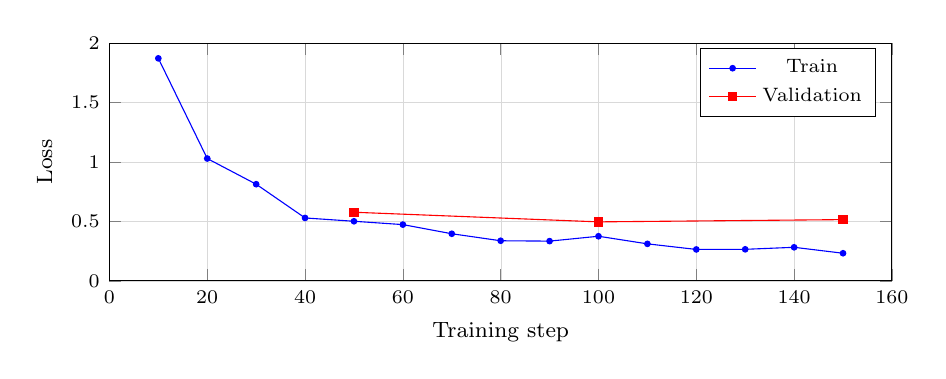
\begin{tikzpicture}
\begin{axis}[
  width=0.95\columnwidth, height=4.6cm,
  xlabel={Training step}, ylabel={Loss},
  xmin=0, xmax=160, ymin=0, ymax=2,
  legend style={font=\scriptsize, at={(0.98,0.98)}, anchor=north east},
  tick label style={font=\scriptsize}, label style={font=\footnotesize},
  grid=both, grid style={line width=.1pt, draw=gray!30}
]
\addplot[blue, mark=*, mark size=1pt] coordinates {
(10,1.872) (20,1.029) (30,0.813) (40,0.529) (50,0.501) (60,0.473) (70,0.396)
(80,0.337) (90,0.334) (100,0.375) (110,0.311) (120,0.264) (130,0.265) (140,0.282) (150,0.232)};
\addlegendentry{Train}
\addplot[red, mark=square*, mark size=1.5pt] coordinates {(50,0.577) (100,0.496) (150,0.515)};
\addlegendentry{Validation}
\end{axis}
\end{tikzpicture}
\caption{Fine-tuning loss; validation loss every 50 steps.}
\label{fig:loss}
\end{figure}

%==============================================================
\section{Evaluation Methodology}

\subsection{Systems}
Table~\ref{tab:systems} lists the six systems. S2/S5 and S4/S6 differ only in the adapter.

\begin{table}[t]
\caption{Systems compared.}
\label{tab:systems}
\centering
\begin{tabular}{lll}
\toprule
ID & Generator & Retrieval \\
\midrule
S1 & Cloud (gpt-oss-20b) & no \\
S2 & Fine-tuned Qwen2.5-1.5B & no \\
S5 & Base Qwen2.5-1.5B & no \\
S3 & Cloud (gpt-oss-20b) & yes \\
S4 & Fine-tuned Qwen2.5-1.5B & yes \\
S6 & Base Qwen2.5-1.5B & yes \\
\bottomrule
\end{tabular}
\end{table}

\subsection{Questions and Overlap Check}
The gold bank has 32 textbook questions with reference answers. We compared each with all 762 training and validation questions by normalised exact match, then by BGE similarity ($\ge 0.82$) to select candidates, each confirmed or rejected by an LLM check of whether the two questions would receive essentially the same answer. This conservative check flagged \textbf{15 of 32} questions (3 verbatim copies, 12 paraphrases), which we excluded. We evaluate the remaining \textbf{17} (11 conceptual, 6 numerical). The check can over-flag topic neighbours, so the clean set is, if anything, harder for the fine-tuned systems.

\subsection{Metrics and Judge}
We use RAGAS~\cite{es2024ragas} 0.4.3: \emph{faithfulness} (claims supported by the retrieved context), \emph{answer relevancy} and \emph{context precision} with reference. Faithfulness and context precision need retrieved context and are undefined for S1, S2 and S5. The judge is \texttt{gpt-oss-120b} through the Groq API; because daily quotas ran out, calls were spread over three API keys from at least two organisations, always with the same judge model. We report means with 95\% bootstrap confidence intervals over questions, and paired differences over questions scored for both systems. Context precision depends on the reference answers; we found three of them wrong (see Section~\ref{sec:integrity}) and re-scored those rows.

\subsection{Calculation Benchmark}
To measure correctness without a judge, we generated page-replacement (FIFO, LRU, optimal), disk-scheduling (FCFS, SSTF, LOOK) and CPU-scheduling (FCFS, SJF, round robin) problems with a fixed seed. Ground truth comes from deterministic simulators, which reproduce the textbook's 15/12/9 page-fault example. Wording differs from the training templates. Forty-five problems were generated and the first three per algorithm were used (27 problems) because local generation was slow; selection is deterministic. S1, S2 and S5 answered without retrieval. An answer is \emph{strictly} correct if its last number equals the truth, and \emph{leniently} correct if the truth appears among the numbers in its last 250 characters.

\subsection{Data Integrity}
\label{sec:integrity}
Nineteen of the 68 answers of S1--S4 had to be regenerated (none of S5/S6): eighteen cloud answers stored the provider's rate-limit error text because a daily token quota was exhausted during generation, and one cloud answer was empty. Scores computed from error text were discarded before final scoring; one further empty cloud answer in the benchmark was also regenerated. Three gold reference answers were incorrect: for the string \texttt{7 0 1 2 0 3 0 4 2 3 0 3 2} with three frames the correct page-fault counts are 10 (FIFO), 9 (LRU) and 7 (OPT), not 9, 8 and 6. We corrected them; re-scoring changed none of the six affected context-precision values. One system (S3) replied with a refusal to a numerical question; the judge cannot score a refusal, so we recorded answer relevancy 0.0, faithfulness as not applicable, and context precision from the identical retrieval of S4. Section~\ref{sec:results} shows how much this single rule matters.

%==============================================================
\section{Results}
\label{sec:results}

\subsection{Text Quality on the 17 Clean Questions}
Table~\ref{tab:main} and Fig.~\ref{fig:bars} give the main results; Table~\ref{tab:paired} gives paired differences.

\begin{table*}[t]
\caption{RAGAS scores on the 17 clean questions: mean [95\% bootstrap CI]. n/a: undefined without retrieval. S3 faithfulness has n=16 (one refusal).}
\label{tab:main}
\centering
\begin{tabular}{llccc}
\toprule
 & System & Faithfulness & Answer relevancy & Context precision \\
\midrule
S1 & Cloud only & n/a & 0.93 [0.91, 0.95] & n/a \\
S2 & Fine-tuned only & n/a & 0.81 [0.76, 0.86] & n/a \\
S5 & Base Qwen only & n/a & 0.94 [0.93, 0.96] & n/a \\
S3 & RAG + cloud & 0.61 [0.42, 0.79] & 0.87 [0.75, 0.94] & 0.57 [0.36, 0.78] \\
S4 & RAG + fine-tuned & 0.32 [0.16, 0.49] & 0.88 [0.84, 0.91] & 0.60 [0.38, 0.80] \\
S6 & RAG + base Qwen & 0.43 [0.26, 0.61] & 0.95 [0.92, 0.97] & 0.60 [0.39, 0.80] \\
\bottomrule
\end{tabular}
\end{table*}

\begin{figure}[t]
\centering
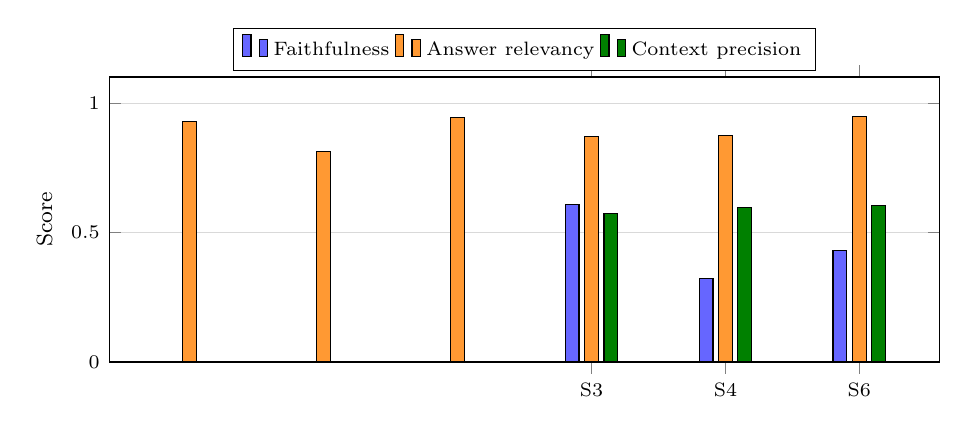
\begin{tikzpicture}
\begin{axis}[
  ybar, width=\columnwidth, height=5.2cm,
  bar width=5pt, ymin=0, ymax=1.1,
  symbolic x coords={S1,S2,S5,S3,S4,S6}, xtick=data,
  ylabel={Score}, tick label style={font=\scriptsize}, label style={font=\footnotesize},
  legend style={font=\scriptsize, at={(0.5,1.02)}, anchor=south, legend columns=3},
  enlarge x limits=0.12, ymajorgrids=true, grid style={line width=.1pt, draw=gray!30}
]
\addplot[fill=blue!60] coordinates {(S3,0.609) (S4,0.321) (S6,0.429)};
\addplot[fill=orange!80] coordinates {(S1,0.929) (S2,0.814) (S5,0.944) (S3,0.872) (S4,0.876) (S6,0.946)};
\addplot[fill=green!50!black] coordinates {(S3,0.574) (S4,0.598) (S6,0.603)};
\legend{Faithfulness, Answer relevancy, Context precision}
\end{axis}
\end{tikzpicture}
\caption{Mean scores per system (17 clean questions). Faithfulness and context precision are undefined for S1, S2 and S5.}
\label{fig:bars}
\end{figure}

\begin{table}[t]
\caption{Paired differences (first minus second) with 95\% bootstrap CI. F: faithfulness, R: answer relevancy.}
\label{tab:paired}
\centering
\small
\setlength{\tabcolsep}{3pt}
\begin{tabular}{llc}
\toprule
Comparison & Metric & Difference [CI] \\
\midrule
S4 $-$ S3 (fine-tuned vs cloud, RAG) & F & $-0.27$ [$-0.45$, $-0.11$] \\
S4 $-$ S3 & R & $+0.00$ [$-0.08$, $+0.14$] \\
\quad same, refusal question dropped & R & $-0.06$ [$-0.10$, $-0.02$] \\
S4 $-$ S6 (fine-tuning, with RAG) & F & $-0.11$ [$-0.29$, $+0.05$] \\
S4 $-$ S6 & R & $-0.07$ [$-0.11$, $-0.03$] \\
S2 $-$ S5 (fine-tuning, no RAG) & R & $-0.13$ [$-0.19$, $-0.08$] \\
S6 $-$ S5 (RAG on base model) & R & $+0.00$ [$-0.01$, $+0.02$] \\
S4 $-$ S2 (RAG on fine-tuned) & R & $+0.06$ [$-0.00$, $+0.13$] \\
S2 $-$ S1 (fine-tuned vs cloud) & R & $-0.12$ [$-0.18$, $-0.06$] \\
\bottomrule
\end{tabular}
\end{table}

The main findings are:
\begin{itemize}
  \item \textbf{The cloud model with retrieval is the most faithful.} S4 is $0.27$ lower than S3 (interval excludes zero).
  \item \textbf{Fine-tuning did not improve these metrics.} Against the same base model, the fine-tuned model has lower answer relevancy without retrieval ($-0.13$) and with retrieval ($-0.07$), and its faithfulness is not detectably higher (S4 $-$ S6 $= -0.11$, interval includes zero).
  \item \textbf{Retrieval changed little} for the base model (S6 $-$ S5 $\approx 0$) or the cloud model (S3 $-$ S1 $=-0.06$, interval includes zero). Context precision is about 0.57--0.60 for all three RAG systems, with no detectable differences; retrieval is weak in absolute terms.
  \item \textbf{The S3--S4 relevancy comparison depends on one scoring rule.} Counting S3's single refusal as 0 gives a tie; dropping that question gives S4 $0.06$ lower (Table~\ref{tab:paired}).
\end{itemize}

\subsection{Calculation Benchmark}
Table~\ref{tab:bench} gives accuracy on the 27 problems. The cloud model solves most of them; both Qwen variants mostly fail. Fine-tuned Qwen is correct on more problems than base Qwen under the lenient criterion (8 versus 4; they disagree on six problems, five in favour of the fine-tuned model), but a sign test gives $p=0.22$, so we do not claim a gain. By category (lenient, out of 9), the cloud model scored 7 (CPU scheduling), 9 (disk) and 7 (page replacement); fine-tuned Qwen 2, 1 and 5; base Qwen 1, 0 and 3. Manual inspection confirmed that Qwen's failures are genuine procedural or arithmetic errors, for example computing each seek distance from the head's starting position. Qwen output is capped at 256 tokens, which truncated some long solutions and may understate its accuracy.

\begin{table}[t]
\caption{Calculation accuracy, 27 problems, no retrieval: correct/total = proportion [95\% Wilson CI].}
\label{tab:bench}
\centering
\small
\setlength{\tabcolsep}{3pt}
\begin{tabular}{lcc}
\toprule
System & Strict (last number) & Lenient (final 250 chars) \\
\midrule
S1 Cloud & 22/27 = 0.81 [0.63, 0.92] & 23/27 = 0.85 [0.68, 0.94] \\
S2 Fine-tuned & 1/27 = 0.04 [0.01, 0.18] & 8/27 = 0.30 [0.16, 0.48] \\
S5 Base Qwen & 0/27 = 0.00 [0.00, 0.12] & 4/27 = 0.15 [0.06, 0.32] \\
\bottomrule
\end{tabular}
\end{table}

\subsection{Latency}
Table~\ref{tab:lat} gives median time per answer on a CPU-only laptop. The local models take tens of seconds per answer, against a few seconds for the cloud model. These are single-run figures; means were inflated by stalls when the machine slept or ran on battery power, so we report medians.

\begin{table}[t]
\caption{Median latency per answer (seconds), single run, CPU only.}
\label{tab:lat}
\centering
\begin{tabular}{lcccccc}
\toprule
 & S1 & S2 & S5 & S3 & S4 & S6 \\
\midrule
Median (s) & 1.2 & 28.2 & 37.4 & 1.9 & 55.9 & 48.3 \\
\bottomrule
\end{tabular}
\end{table}

%==============================================================
\section{Discussion}

\textbf{What the data support.} The cloud model with retrieval is clearly the most faithful system. The 1.5B model benefited neither in text quality nor, detectably, in calculation accuracy from our fine-tuning. We did not test why. A plausible hypothesis is that the fine-tuned model answers tersely in a textbook style while the relevancy metric favours longer, more generic answers; the training prompt also differs from the inference prompt, and the adapter was trained on a 4-bit base but run in 32-bit precision. These explanations are untested.

\textbf{Dataset implications.} The dataset's numerical half is highly templated (nine question openings), its passages are short and repeated, and its conceptual categories are small. These properties may limit what a model can learn from it, but the study does not isolate them.

\textbf{Pitfalls.} Several implementation details changed results more than model choice, and we record them for others. (i) A strong repetition penalty and an n-gram ban, which also apply to the prompt, prevented the model from quoting retrieved text and produced incoherent answers in an early run. (ii) Chains kept conversation memory, so one system's answer leaked into the next system's prompt. (iii) Rate-limit error messages and empty completions were stored as answers. (iv) One API path returned no retrieved context, which would have scored faithfulness against nothing. (v) Three gold reference answers were wrong. (vi) Judge token quotas truncated scoring runs. None of these is visible from aggregate scores alone.

\subsection{Limitations}
\begin{itemize}
  \item \textbf{Small clean set.} Seventeen questions (six numerical) and 27 calculation problems give wide intervals; only large differences are detectable.
  \item \textbf{Single judge, no human evaluation.} The judge is one LLM, and judge access was split across several API keys; no human ratings were collected.
  \item \textbf{Same-family bias.} A judge from the Qwen family would be expected to favour Qwen-based systems, so the cloud model's lead on faithfulness is conservative; we did not measure this bias.
  \item \textbf{Calculation coverage.} Correctness of RAG systems and of the full question set was not measured; the benchmark covers three problem families without retrieval, and Qwen output was capped at 256 tokens.
  \item \textbf{Overlap check is approximate.} It relies on an LLM judgement and may over- or under-flag.
  \item \textbf{Prompt and precision mismatch,} and a single CPU-only machine for latency.
  \item \textbf{One textbook, one adapter,} trained once; we did not vary training settings or compare checkpoints.
\end{itemize}

%==============================================================
\section{Conclusion and Future Work}
On 17 questions that do not overlap the training data, retrieval with a 20B cloud model was the most faithful configuration, and a LoRA adapter trained on our 762-example dataset did not improve a 1.5B model's text quality and did not significantly improve its calculation accuracy. The study's main value is therefore comparative and methodological: a documented dataset and adapter, a judge-free calculation benchmark, and an evaluation protocol that exposed several silent failure modes. Future work: a larger clean test set with human ratings and a second judge from another model family; a more diverse and larger training set built from retrieved chunks; matching training and inference prompts and comparing checkpoints; longer generation limits for calculations; and stronger retrieval, since context precision is the weakest metric.

\section*{Reproducibility}
Code, dataset files, the adapter, raw answers, scores and the benchmark are in the project repository, with a write-up of every setting and correction. Replace this paragraph with the public repository or dataset link before submission.

\begin{thebibliography}{00}
\bibitem{lewis2020rag} P.~Lewis \emph{et al.}, ``Retrieval-augmented generation for knowledge-intensive NLP tasks,'' in \emph{Advances in Neural Information Processing Systems (NeurIPS)}, 2020.
\bibitem{hu2022lora} E.~J. Hu \emph{et al.}, ``LoRA: Low-rank adaptation of large language models,'' in \emph{Int. Conf. on Learning Representations (ICLR)}, 2022.
\bibitem{dettmers2023qlora} T.~Dettmers, A.~Pagnoni, A.~Holtzman, and L.~Zettlemoyer, ``QLoRA: Efficient finetuning of quantized LLMs,'' in \emph{Advances in Neural Information Processing Systems (NeurIPS)}, 2023.
\bibitem{es2024ragas} S.~Es, J.~James, L.~Espinosa-Anke, and S.~Schockaert, ``RAGAS: Automated evaluation of retrieval augmented generation,'' in \emph{Proc. EACL: System Demonstrations}, 2024.
\bibitem{zheng2023judge} L.~Zheng \emph{et al.}, ``Judging LLM-as-a-judge with MT-Bench and Chatbot Arena,'' in \emph{NeurIPS Datasets and Benchmarks Track}, 2023.
\bibitem{ji2023hallucination} Z.~Ji \emph{et al.}, ``Survey of hallucination in natural language generation,'' \emph{ACM Computing Surveys}, vol.~55, no.~12, 2023.
\bibitem{gao2023ragsurvey} Y.~Gao \emph{et al.}, ``Retrieval-augmented generation for large language models: A survey,'' arXiv:2312.10997, 2023.
\bibitem{qwen25} Qwen Team, ``Qwen2.5 technical report,'' arXiv:2412.15115, 2024.
\bibitem{xiao2023cpack} S.~Xiao \emph{et al.}, ``C-Pack: Packaged resources to advance general Chinese embedding,'' arXiv:2309.07597, 2023.
\bibitem{gptoss} OpenAI, ``gpt-oss-120b and gpt-oss-20b model card,'' arXiv:2508.10925, 2025.
\bibitem{galvin} A.~Silberschatz, P.~B. Galvin, and G.~Gagne, \emph{Operating System Concepts}. Hoboken, NJ, USA: Wiley.
\end{thebibliography}

\end{document}
